% Slides for Chapter 1 of the BARCS student guide: the ideas.
% Build in this folder: pdflatex barcs_slides_ch1.tex (run twice).
\documentclass[aspectratio=169,11pt]{beamer}
% Shared preamble for the BARCS student-guide slides (Beamer, metropolis).
% The slides follow the two-chapter textbook in ../chapter1 and ../chapter2:
% each section is one textbook step with the same title, and the worked
% examples use the same numbers. Short sentences, as in the textbook
% (ASD-STE100 style). No quiz: the quizzes stay in the textbook.
\usetheme[progressbar=frametitle,sectionpage=progressbar,numbering=fraction]{metropolis}
\usepackage[T1]{fontenc}
\usepackage{lmodern}
\usepackage{amsmath,amssymb}
\usepackage{booktabs}
\usepackage[most]{tcolorbox}
\usepackage{tikz}
\usetikzlibrary{arrows.meta,positioning}

\definecolor{barcsblue}{HTML}{0072B2}
\definecolor{barcsgreen}{HTML}{009E73}
\definecolor{barcsorange}{HTML}{D55E00}
\definecolor{barcsdark}{HTML}{1F3B4D}
\setbeamercolor{frametitle}{bg=barcsdark,fg=white}
\setbeamercolor{progress bar}{fg=barcsorange,bg=barcsdark!30}
\setbeamercolor{title separator}{fg=barcsorange}
\setbeamercolor{alerted text}{fg=barcsorange}
\setbeamercolor{normal text}{fg=black!85}

% The same three boxes as the textbook.
\newtcolorbox{symbols}[1][What the symbols mean]{colback=barcsblue!5,colframe=barcsblue,
  fonttitle=\bfseries\small,title=#1,boxrule=0.6pt,arc=2pt,left=4pt,right=4pt,top=2pt,bottom=2pt}
\newtcolorbox{worked}[1][]{colback=barcsgreen!6,colframe=barcsgreen!80!black,
  fonttitle=\bfseries\small,title=Worked example#1,boxrule=0.6pt,arc=2pt,left=4pt,right=4pt,top=2pt,bottom=2pt}
\newtcolorbox{remember}{colback=barcsorange!6,colframe=barcsorange,
  fonttitle=\bfseries\small,title=Remember,boxrule=0.6pt,arc=2pt,left=4pt,right=4pt,top=2pt,bottom=2pt}

\author{Prepared for Hyun-Hwan Jeong and Kyu-Won Lee}
\date{Companion slides to the student guide \quad$\cdot$\quad BARCS 0.2.1 \quad$\cdot$\quad Grades 7 to 9}

% The four-library example used in both chapters.
\newcommand{\datatable}{%
\begin{tabular}{lcrr}
\toprule
Library & Group & Guide count $K$ & Total count $N$\\
\midrule
1 & control & 180 & 1{,}000{,}000\\
2 & control & 240 & 1{,}200{,}000\\
3 & drug    & 120 & 1{,}000{,}000\\
4 & drug    &  80 &   800{,}000\\
\bottomrule
\end{tabular}}

\title{How BARCS Finds Important Genes}
\subtitle{Chapter 1: The ideas}

\begin{document}

\maketitle

\begin{frame}{The plan for Chapter 1}
\begin{columns}[T]
\begin{column}{0.55\textwidth}
\begin{enumerate}
\item The experiment: a CRISPR screen
\item The data
\item Step 1: Turn counts into proportions
\item Step 2: Compare the groups with a fold change
\item Step 3: Odds and log-odds
\item Step 4: Two kinds of noise
\item Step 5: The design matrix
\end{enumerate}
\end{column}
\begin{column}{0.4\textwidth}
\begin{remember}
Each section of these slides has the same title as a section of the
textbook. The examples use the same numbers.
\end{remember}
\end{column}
\end{columns}
\end{frame}

%=====================================================================
\section{The experiment: a CRISPR screen}
%=====================================================================

\begin{frame}{What scientists want to know}
\begin{itemize}
\item Each cell has about 20{,}000 genes.
\item A gene is a set of instructions.
\item Question: which genes does a cell need, for example to survive a
  cancer drug?
\end{itemize}
\bigskip
A \alert{CRISPR screen} tests thousands of genes at the same time.
\end{frame}

\begin{frame}{A CRISPR screen in four steps}
\begin{enumerate}
\item Make a \alert{library} of short pieces of RNA, called \alert{guides}.
  Each guide switches off one gene.
\item Put one guide into each cell. Now each cell has one gene switched off.
\item Grow the cells: some in normal conditions (\alert{control}), some
  with a drug (\alert{drug}).
\item A sequencing machine counts each guide. This number is a
  \alert{read count}.
\end{enumerate}
\medskip
\begin{center}
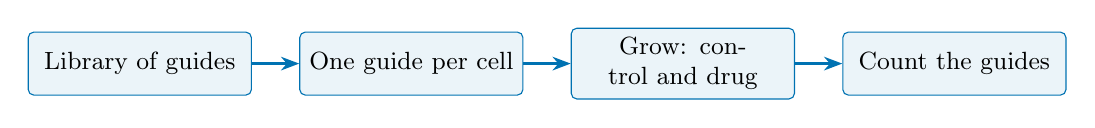
\begin{tikzpicture}[node distance=6mm,
  st/.style={draw=barcsblue,fill=barcsblue!8,rounded corners=2pt,align=center,
             minimum height=8mm,text width=2.6cm,font=\small},
  ar/.style={-{Stealth},thick,barcsblue}]
\node[st] (a) {Library of guides};
\node[st,right=of a] (b) {One guide per cell};
\node[st,right=of b] (c) {Grow: control and drug};
\node[st,right=of c] (d) {Count the guides};
\draw[ar] (a)--(b); \draw[ar] (b)--(c); \draw[ar] (c)--(d);
\end{tikzpicture}
\end{center}
\end{frame}

\begin{frame}{Why a count tells us about a gene}
\begin{itemize}
\item Suppose cells need a gene to survive the drug.
\item Cells that lose that gene die.
\item So their guide becomes \alert{rare} in the drug group.
\end{itemize}
\bigskip
\begin{remember}
BARCS does not look at cells directly. It looks at read counts. A guide
that becomes rare tells us that its gene is important.
\end{remember}
\end{frame}

\begin{frame}{Replicates and libraries}
\begin{itemize}
\item Scientists repeat each group more than one time.
  Each repeat is a \alert{replicate}.
\item Each sample that the machine reads is a \alert{library}.
\item Our example has \alert{four libraries}:
  \begin{itemize}
  \item two control replicates
  \item two drug replicates
  \end{itemize}
\end{itemize}
\end{frame}

%=====================================================================
\section{The data}
%=====================================================================

\begin{frame}{Read counts for one guide}
\centering
\datatable

\smallskip
\small We use these numbers on every slide.
\medskip

\begin{symbols}
\small
$K$: the read count of one guide in one library (library~1: $K = 180$).\quad
$N$: the total read count of one library (library~1: $N = 1{,}000{,}000$).\quad
$i$: the library number ($K_2 = 240$).
\end{symbols}
\end{frame}

\begin{frame}{Record the totals first}
\begin{remember}
Always record $N$ \emph{before} you remove any guides from the table.

If you remove guides first, the totals become wrong. Then all the later
numbers become wrong too.
\end{remember}
\end{frame}

%=====================================================================
\section{Step 1: Turn counts into proportions}
%=====================================================================

\begin{frame}{Divide each count by its library total}
\begin{itemize}
\item Library 2 has more reads only because the machine read it more.
\item So we cannot compare raw counts.
\item Divide each count by its total. The result is a \alert{proportion}:
\end{itemize}
\[
p = \frac{K}{N}
\]
\begin{itemize}
\item Proportions are tiny. Multiply by one million: \alert{per million}
  reads.
\end{itemize}
\begin{symbols}
\small $p$: the proportion of all reads that belong to the guide. Always
between 0 and 1.
\end{symbols}
\end{frame}

\begin{frame}{Worked example: proportions}
\begin{worked}[ 1]
\small
\begin{tabular}{@{}lll@{}}
Library 1: & $180 \div 1{,}000{,}000 = 0.000180$ & $= 180$ per million\\
Library 2: & $240 \div 1{,}200{,}000 = 0.000200$ & $= 200$ per million\\
Library 3: & $120 \div 1{,}000{,}000 = 0.000120$ & $= 120$ per million\\
Library 4: & $\phantom{0}80 \div \phantom{0,}800{,}000 = 0.000100$ & $= 100$ per million\\
\end{tabular}
\end{worked}
\begin{itemize}
\item Control: 180 and 200 per million.
\item Drug: 120 and 100 per million.
\item The guide is \alert{less common} with the drug.
\end{itemize}
\end{frame}

%=====================================================================
\section{Step 2: Compare the groups with a fold change}
%=====================================================================

\begin{frame}{Combine the replicates of each group}
Add the counts and add the totals of each group:
\[
p_{\text{control}} = \frac{180+240}{1{,}000{,}000+1{,}200{,}000}
 = \frac{420}{2{,}200{,}000} = 0.000191 \quad (191 \text{ per million})
\]
\[
p_{\text{drug}} = \frac{120+80}{1{,}000{,}000+800{,}000}
 = \frac{200}{1{,}800{,}000} = 0.000111 \quad (111 \text{ per million})
\]
\end{frame}

\begin{frame}{The fold change}
\[
\text{fold change} = \frac{p_{\text{drug}}}{p_{\text{control}}}
 = \frac{0.000111}{0.000191} = 0.58
\]
The guide keeps only 58\% of its control level. It loses 42\%.
\medskip
\begin{remember}
\begin{itemize}
\item Fold change $= 1$: no change.
\item Fold change $< 1$: the guide becomes rarer. Cells may need this gene.
\item Fold change $> 1$: the guide becomes more common. Losing this gene may
  help the cells.
\end{itemize}
\end{remember}
\end{frame}

\begin{frame}{Logarithms make changes symmetric}
\begin{itemize}
\item ``Double'' is a fold change of 2. ``Half'' is 0.5.
\item Same size of change, but 2 and 0.5 do not look equal.
\item The \alert{base-2 logarithm}, $\log_2$, counts how many times you
  double.
\end{itemize}
\begin{center}
\begin{tabular}{lccccc}
\toprule
Fold change & 0.25 & 0.5 & 1 & 2 & 4\\
$\log_2$(fold change) & $-2$ & $-1$ & 0 & 1 & 2\\
\bottomrule
\end{tabular}
\end{center}
Now ``double'' is $+1$ and ``half'' is $-1$.
\end{frame}

\begin{frame}{Worked example: log fold change}
\begin{worked}[ 2]
Our fold change is 0.58, between 0.5 and 1.
So $\log_2(0.58)$ is between $-1$ and 0.

A calculator gives $\log_2(0.58) = -0.78$: the guide drops by 0.78
``halvings''.
\end{worked}
\begin{itemize}
\item BARCS uses the \alert{natural logarithm}, $\ln$: powers of
  $e = 2.718\ldots$ instead of powers of 2.
\item To go back: if $\ln(x) = b$, then $x = e^{b}$.
\item For our guide: $\ln(0.58) = -0.54$.
\end{itemize}
\end{frame}

%=====================================================================
\section{Step 3: Odds and log-odds}
%=====================================================================

\begin{frame}{Odds and log-odds}
The \alert{odds} compare the reads of the guide with all other reads:
\[
\text{odds} = \frac{p}{1-p}
\]
The \alert{log-odds} is the natural logarithm of the odds:
\[
\text{log-odds} = \ln\!\left(\frac{p}{1-p}\right)
\]
\end{frame}

\begin{frame}{Worked example: odds and log-odds}
\begin{worked}[ 3]
Control: $p = 0.000191$, so odds $= 0.000191 \div 0.999809 = 0.000191$.

For small $p$, the odds and the proportion are almost equal, because $1-p$
is almost 1.

\begin{tabular}{@{}ll@{}}
Log-odds, control: & $\ln(0.000191) = -8.56$\\
Log-odds, drug:    & $\ln(0.000111) = -9.10$\\
Difference:        & $-9.10 - (-8.56) = -0.54$\\
\end{tabular}

The difference is the same as $\ln(\text{fold change})$ from Step~2.
\end{worked}
\end{frame}

\begin{frame}{Why use log-odds?}
\begin{remember}
For guides, a difference in log-odds is almost exactly the natural log of
the fold change. So you can read BARCS results as log fold changes.
\end{remember}
\medskip
\begin{itemize}
\item A proportion must stay between 0 and 1.
\item A log-odds can be any number, positive or negative.
\item So BARCS can add effects together safely (Step 5).
\end{itemize}
\end{frame}

%=====================================================================
\section{Step 4: Two kinds of noise}
%=====================================================================

\begin{frame}{Replicates are never equal}
\begin{itemize}
\item The two control libraries gave 180 and 200 per million.
\item This difference is \alert{noise}.
\item BARCS must know the size of the noise to tell a real change from a
  chance change.
\end{itemize}
\medskip
\begin{columns}[T]
\begin{column}{0.48\textwidth}
\begin{block}{1. Counting noise}
The machine reads a random sample. Like a handful from a bag of a million
marbles: the number of red marbles changes each time.
\end{block}
\end{column}
\begin{column}{0.48\textwidth}
\begin{block}{2. Biological noise}
Each replicate is a different group of living cells. The cells grow a
little differently each time.
\end{block}
\end{column}
\end{columns}
\end{frame}

\begin{frame}{Variance: the plan}
\begin{itemize}
\item \alert{Variance}: the average squared distance from the expected
  value.
\item \alert{Standard deviation}: the square root of the variance, in the
  units of the counts.
\item The sign $\times$ means ``multiply''. $N \times \mu$ is ``$N$ times
  $\mu$''. It is \alert{not} one symbol.
\end{itemize}
\medskip
We build the formula in four parts: (1) the expected count, (2) counting
noise, (3) biological noise, (4) add the two parts.
\medskip
\begin{symbols}
\small
$N$: library total ($1{,}000{,}000$).\quad
$\mu$ (``mu''): expected proportion (control: $0.000191$).\quad
$\rho$ (``rho''): size of the biological noise.
\end{symbols}
\end{frame}

\begin{frame}{Part 1: The expected count}
\begin{itemize}
\item The machine reads $N$ reads.
\item Each read belongs to our guide with the chance $\mu$.
\end{itemize}
\[
\text{expected count} = N \times \mu
\]
\begin{worked}[ 4a]
$N \times \mu = 1{,}000{,}000 \times 0.000191 = 191$ reads.

The real counts are near 191, but not exactly 191. The variance tells how
far they normally are.
\end{worked}
\end{frame}

\begin{frame}{Part 2: One read --- five marbles}
One red marble (value 1), four blue (value 0). Chance of red $\mu = 0.2$.
Average $= 0.2$.
\medskip

\begin{columns}[T]
\begin{column}{0.55\textwidth}
\small
\begin{tabular}{@{}lccc@{}}
\toprule
Marble & Value & Distance & Squared\\
\midrule
red & 1 & $+0.8$ & 0.64\\
blue & 0 & $-0.2$ & 0.04\\
blue & 0 & $-0.2$ & 0.04\\
blue & 0 & $-0.2$ & 0.04\\
blue & 0 & $-0.2$ & 0.04\\
\midrule
Sum & & \alert{0} & 0.80\\
Average & & 0 & \textbf{0.16}\\
\bottomrule
\end{tabular}
\end{column}
\begin{column}{0.42\textwidth}
\begin{itemize}
\item Plain distances \alert{cancel}: the sum is always 0.
\item Squares are never negative, so they do not cancel.
\item Average squared distance $= 0.80 / 5 = 0.16$.
\item This is the \alert{variance}.
\end{itemize}
\end{column}
\end{columns}
\end{frame}

\begin{frame}{Why squares? Because squared spreads add up}
Two fair coins (heads $= 1$, $\mu = 0.5$). Four equally likely results:
\medskip

\begin{columns}[T]
\begin{column}{0.48\textwidth}
\small
\begin{tabular}{@{}lccc@{}}
\toprule
Coins & Total & Dist.\ from 1 & Squared\\
\midrule
T, T & 0 & $-1$ & 1\\
T, H & 1 & 0 & 0\\
H, T & 1 & 0 & 0\\
H, H & 2 & $+1$ & 1\\
\bottomrule
\end{tabular}
\end{column}
\begin{column}{0.50\textwidth}
\small
\begin{tabular}{@{}lcc@{}}
\toprule
& Squared & Size only\\
\midrule
One coin & 0.25 & 0.5\\
One + one & 0.5 & 1.0\\
Total of two & 0.5 & 0.5\\
\midrule
Adds up? & \alert{yes} & no\\
\bottomrule
\end{tabular}
\end{column}
\end{columns}
\medskip
\begin{itemize}\small
\item We add a million reads (Part 2) and two kinds of noise (Part 4). We
  need a spread that adds up.
\item R.\,A. Fisher named this the \emph{variance} in 1918 for this reason.
  Squared distances go back to Legendre's ``least squares'' (1805).
\end{itemize}
\end{frame}

\begin{frame}{The general formula for one read}
Replace ``one in five'' by any chance $\mu$:
\medskip

\begin{tabular}{@{}lccc@{}}
\toprule
Value & How often & Distance from $\mu$ & Squared distance\\
\midrule
1 & $\mu$ & $1-\mu$ & $(1-\mu)^2$\\
0 & $1-\mu$ & $-\mu$ & $\mu^2$\\
\bottomrule
\end{tabular}
\medskip

Average squared distance $=$ (squared distance $\times$ how often), added:
\[
\text{variance of one read} = \mu \times (1-\mu)^2 + (1-\mu) \times \mu^2
\]
\begin{worked}[ 4b: five marbles again]
$0.2 \times 0.8^2 + 0.8 \times 0.2^2 = 0.128 + 0.032 = 0.16$ --- the same as
the table.
\end{worked}
\end{frame}

\begin{frame}{Open the square}
A square means ``multiply by itself'':
\[
(1-\mu)^2 = (1-\mu) \times (1-\mu)
\]
Multiply each part of the first bracket by each part of the second:
\[
(1-\mu) \times (1-\mu) = 1 \times 1 \;-\; 1 \times \mu \;-\; \mu \times 1
 \;+\; \mu \times \mu = 1 - 2 \times \mu + \mu^2
\]
\begin{worked}[ 4b: check with numbers]
With $\mu = 0.2$: $0.8 \times 0.8 = 0.64$\qquad and\qquad $1 - 2 \times 0.2 + 0.04 = 0.64$.
\end{worked}
\end{frame}

\begin{frame}{From the long formula to $\mu \times (1-\mu)$}
\footnotesize
\renewcommand{\arraystretch}{1.25}
\begin{tabular}{@{}r@{\;}l l l@{}}
\toprule
& With letters & With $\mu = 0.2$ & What we did\\
\midrule
1. & $\mu \times (1-\mu)^2 + (1-\mu) \times \mu^2$ & $0.128 + 0.032$ & start\\
2. & $\mu \times (1 - 2\times\mu + \mu^2) + (1-\mu) \times \mu^2$ & $0.128 + 0.032$ & open the square\\
3. & $(\mu - 2\times\mu^2 + \mu^3) + (\mu^2 - \mu^3)$ & $(0.2 - 0.08 + 0.008) + (0.04 - 0.008)$ & multiply in\\
4. & $\mu - 2\times\mu^2 + \mu^2 + \mu^3 - \mu^3$ & $0.2 - 0.08 + 0.04 + 0.008 - 0.008$ & sort the powers\\
5. & $\mu - \mu^2$ & $0.2 - 0.04 = 0.16$ & combine\\
6. & $\mu \times (1-\mu)$ & $0.2 \times 0.8 = 0.16$ & take $\mu$ out\\
\bottomrule
\end{tabular}
\medskip

\normalsize
Every line gives \alert{0.16}. Shorter way: take out the common part
$\mu \times (1-\mu)$:
\[
\mu \times (1-\mu) \times \bigl[(1-\mu) + \mu\bigr] = \mu \times (1-\mu) \times 1
\]
\end{frame}

\begin{frame}{Part 2: Counting noise for $N$ reads}
\begin{itemize}
\item The reads are independent. Variances of independent values
  \alert{add up}.
\item $N$ reads: $N$ times the variance of one read.
\end{itemize}
\[
\text{counting noise} = N \times \mu \times (1-\mu)
\]
\begin{worked}[ 4c: many reads]
\textbf{100 reads, $\mu = 0.2$:} expected $100 \times 0.2 = 20$; variance
$100 \times 0.16 = 16$; SD $\sqrt{16} = 4$.\\
Ten repeats gave 17, 19, 21, 25, 17, 25, 27, 22, 21, 14: near 20, about 4
away.

\textbf{Our guide:} $1{,}000{,}000 \times 0.000191 \times 0.999809 = 191$.
\end{worked}
\end{frame}

\begin{frame}{Part 3: What is the wobble?}
\begin{itemize}\small
\item Each replicate is different living cells. So the \alert{true
  proportion} $p$ of the guide is a little different in each replicate.
\item The \alert{wobble} is how far $p$ moves from its average $\mu$:
  \quad $V = $ average of $(p - \mu)^2$.
\end{itemize}
\begin{center}
\resizebox{!}{0.46\textheight}{% The wobble of the true proportion p between replicates (mu = 0.2).
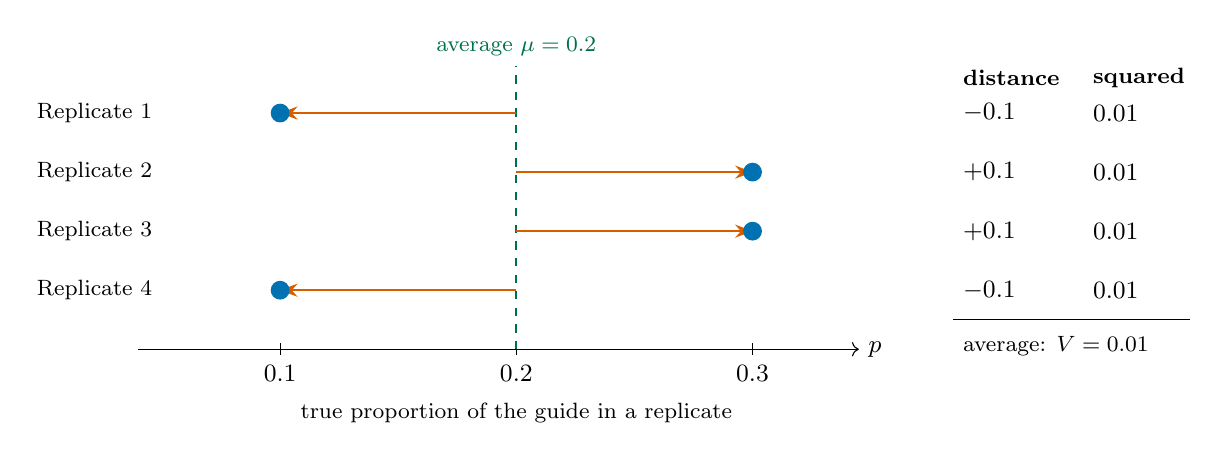
\begin{tikzpicture}[x=30cm,y=0.75cm,font=\small,
  dot/.style={circle,fill=barcsblue,inner sep=2.4pt},
  dist/.style={-{Stealth[length=2.2mm]},thick,barcsorange}]
  % axis
  \draw[->] (0.04,0) -- (0.345,0) node[right] {$p$};
  \foreach \t in {0.1,0.2,0.3} \draw (\t,0.1) -- (\t,-0.1) node[below] {\t};
  \node[below,align=center,font=\footnotesize] at (0.2,-0.75)
    {true proportion of the guide in a replicate};
  % mean line
  \draw[dashed,barcsgreen!70!black,thick] (0.2,0) -- (0.2,4.8)
    node[above,font=\footnotesize,align=center] {average $\mu = 0.2$};
  % header
  \node[font=\footnotesize\bfseries,anchor=west] at (0.385,4.6) {distance};
  \node[font=\footnotesize\bfseries,anchor=west] at (0.44,4.6) {squared};
  % replicates
  \foreach \y/\p/\d/\s in {4/0.1/{$-0.1$}/0.01, 3/0.3/{$+0.1$}/0.01,
                         2/0.3/{$+0.1$}/0.01, 1/0.1/{$-0.1$}/0.01} {
    \node[anchor=east,font=\footnotesize] at (0.05,\y) {Replicate \the\numexpr5-\y\relax};
    \draw[dist] (0.2,\y) -- (\p,\y);
    \node[dot] at (\p,\y) {};
    \node[anchor=west] at (0.385,\y) {\d};
    \node[anchor=west] at (0.44,\y) {\s};
  }
  \draw (0.385,0.5) -- (0.485,0.5);
  \node[anchor=west,font=\footnotesize] at (0.385,0.05)
    {average: $V = 0.01$};
\end{tikzpicture}
}
\end{center}
{\small No wobble: every replicate at $p = 0.2$, all arrows 0, $V = 0$.}
\end{frame}

\begin{frame}{Where $\rho$ comes from: two reads from one replicate}
Take two reads from the same replicate. \alert{If the first read is our
guide, is the second more likely to be our guide too?}
\medskip
\begin{columns}[T]
\begin{column}{0.48\textwidth}
\begin{block}{No wobble: no}
Every replicate has $p = \mu$.\\
Chance both are our guide $= \mu \times \mu$.\\
The reads are unrelated.
\end{block}
\end{column}
\begin{column}{0.48\textwidth}
\begin{block}{Wobble: yes}
Read 1 is our guide $\Rightarrow$ this replicate probably has a high $p$
$\Rightarrow$ read 2 is more likely our guide.\\
The reads \alert{move together}.
\end{block}
\end{column}
\end{columns}
\medskip
\begin{remember}
$\rho$ is the \alert{correlation} between two reads from the same replicate
(0 = unrelated, 1 = always the same). That is why its name is $\rho$, the
usual letter for a correlation.
\end{remember}
\end{frame}

\begin{frame}{Step 1: how often are both reads our guide?}
In a replicate with true proportion $p$: chance $= p \times p$. Average over
the replicates:
\medskip

\small
\renewcommand{\arraystretch}{1.3}\setlength{\tabcolsep}{4pt}
\begin{tabular}{@{}lcccc@{}}
\toprule
Case ($\mu = 0.2$) & Both our guide & No wobble ($\mu\times\mu$) & Extra & $\rho$ = extra $\div$ 0.16\\
\midrule
A. $p = 0.2$ always & $0.04$ & 0.04 & 0 & 0\\
B. $p = 0.1$ or $0.3$ & $(0.01 + 0.09)/2 = 0.05$ & 0.04 & 0.01 & 0.0625\\
C. $p = 0$ or $1$ & $0.8 \times 0 + 0.2 \times 1 = 0.2$ & 0.04 & 0.16 & 1\\
\bottomrule
\end{tabular}
\normalsize
\medskip

\begin{itemize}
\item The wobble makes ``both are our guide'' \alert{more likely} than
  $\mu \times \mu$.
\item The extra is the \alert{covariance}. It is always equal to the wobble
  $V$ (0, 0.01, 0.16).
\end{itemize}
\end{frame}

\begin{frame}{Step 2a: the chance that both reads are our guide}
\begin{columns}[T]
\begin{column}{0.44\textwidth}
\textbf{Inside one replicate} (true proportion $p$):
\begin{itemize}\small
\item Each read is our guide with chance $p$.
\item Given $p$, the two reads do not affect each other (like two coin
  throws).
\item So: chance both $= p \times p$.
\end{itemize}
{\small Example: $p = 0.3 \Rightarrow 0.3 \times 0.3 = 0.09$.}
\end{column}
\begin{column}{0.52\textwidth}
\textbf{Over all replicates} (case B):
\medskip

\small
\begin{tabular}{@{}lcc@{}}
\toprule
Replicates & $p$ & Both our guide\\
\midrule
half & 0.1 & $0.1 \times 0.1 = 0.01$\\
half & 0.3 & $0.3 \times 0.3 = 0.09$\\
\midrule
average & $\mu = 0.2$ & $(0.01 + 0.09)/2 = \mathbf{0.05}$\\
\bottomrule
\end{tabular}
\end{column}
\end{columns}
\[
\text{chance both reads are our guide} = \text{average of } p \times p = \text{average of } p^2
\]
{\small Without wobble it would be $0.2 \times 0.2 = 0.04$. The wobble makes
it bigger: $0.05$.}
\end{frame}

\begin{frame}{Step 2b: average of $X_1 \times X_2$ $=$ chance both are our guide}
Each read $X$ is 1 (our guide) or 0. The four results:
\medskip

\begin{columns}[T]
\begin{column}{0.5\textwidth}
\small
\begin{tabular}{@{}ccc@{}}
\toprule
$X_1$ & $X_2$ & $X_1 \times X_2$\\
\midrule
1 & 1 & \alert{1}\\
1 & 0 & 0\\
0 & 1 & 0\\
0 & 0 & 0\\
\bottomrule
\end{tabular}
\end{column}
\begin{column}{0.46\textwidth}
\begin{itemize}\small
\item $X_1 \times X_2 = 1$ only when \alert{both} reads are 1.
\item In all other cases it is 0.
\end{itemize}
\end{column}
\end{columns}
\[
\text{avg.\ of } X_1 \times X_2
 = 1 \times (\text{chance both}) + 0 \times (\text{other chances})
 = \text{chance both}
\]
\begin{worked}[ case B]
avg.\ of $X_1 \times X_2 = 0.05$ (Step 2a).
\end{worked}
\end{frame}

\begin{frame}{Step 2c: covariance $=$ average of $p^2 - \mu^2$}
\small
\renewcommand{\arraystretch}{1.1}\setlength{\tabcolsep}{3pt}
\begin{tabular}{@{}l l@{}}
\toprule
\textbf{Line} & \textbf{Why}\\
\midrule
covariance $=$ avg.\ of $(X_1 - \mu) \times (X_2 - \mu)$ & definition\\
$=$ avg.\ of $X_1 \times X_2 - \mu \times X_2 - X_1 \times \mu + \mu \times \mu$ & open the brackets\\
$=$ avg.\ of $X_1 \times X_2 - \mu \times \mu - \mu \times \mu + \mu \times \mu$ & avg.\ of $X_1$ $=$ avg.\ of $X_2$ $= \mu$\\
$=$ avg.\ of $X_1 \times X_2 - \mu \times \mu$ & $-\mu \times \mu + \mu \times \mu = 0$\\
$=$ (chance both reads are our guide) $- \mu \times \mu$ & only $1 \times 1 = 1$ (Step 2b)\\
$=$ (average of $p \times p$) $- \mu \times \mu$ & both $= p \times p$ per replicate (2a)\\
$=$ average of $p^2 - \mu^2$ & $p \times p$ is written $p^2$\\
\bottomrule
\end{tabular}
\begin{worked}[ case B]
avg.\ of $X_1 \times X_2 = 0.05$, so covariance $= 0.05 - 0.04 = 0.01$.
\end{worked}
\end{frame}

\begin{frame}{Step 2d: average of $p^2 - \mu^2$ is the wobble $V$}
\small
\renewcommand{\arraystretch}{1.1}\setlength{\tabcolsep}{3pt}
\begin{tabular}{@{}l l l@{}}
\toprule
\textbf{Line} & \textbf{Why} & \textbf{Case B}\\
\midrule
$V = $ avg.\ of $(p - \mu) \times (p - \mu)$ & definition of $V$ & $0.01$\\
$\phantom{V} = $ avg.\ of $\bigl(p^2 - 2 \times \mu \times p + \mu^2\bigr)$ & multiply out & \\
$\phantom{V} = $ avg.\ of $p^2 - 2 \times \mu \times (\text{avg.\ of } p) + \mu^2$ & average each part & $0.05 - 2 \times 0.2 \times 0.2 + 0.04$\\
$\phantom{V} = $ avg.\ of $p^2 - 2 \times \mu^2 + \mu^2$ & avg.\ of $p$ is $\mu$ & $0.05 - 0.08 + 0.04$\\
$\phantom{V} = $ avg.\ of $p^2 - \mu^2$ & $-2\times\mu^2 + \mu^2 = -\mu^2$ & $0.05 - 0.04 = 0.01$\\
\bottomrule
\end{tabular}
\medskip
\begin{remember}
Step 2c: covariance $=$ avg.\ of $p^2 - \mu^2$.\quad Step 2d: $V = $ avg.\
of $p^2 - \mu^2$.\\
Same right side, so \alert{covariance of two reads $= V$} (case B: both
0.01).
\end{remember}
\end{frame}

\begin{frame}{Step 3: correlation $= \rho$}
\begin{itemize}
\item Correlation (Pearson) $=$ covariance $\div$ (SD of read 1 $\times$ SD
  of read 2).
\item Each read has variance $\mu \times (1-\mu)$ (Part 2), so each SD $=
  \sqrt{\mu \times (1-\mu)}$.
\end{itemize}
\[
\rho = \frac{V}{\sqrt{\mu \times (1-\mu)} \times \sqrt{\mu \times (1-\mu)}}
 = \frac{V}{\mu \times (1-\mu)}
\]
\begin{worked}[ case B]
$\rho = 0.01 \div (0.2 \times 0.8) = 0.01 \div 0.16 = 0.0625$.\\
A computer drew 100{,}000 pairs of reads: correlation 0.06.
\end{worked}
\end{frame}


\begin{frame}{$\rho$ on a meter from 0 to 1}
\begin{center}
\resizebox{!}{0.5\textheight}{% rho = how full the "wobble meter" is; full = mu*(1-mu) (mu = 0.2).
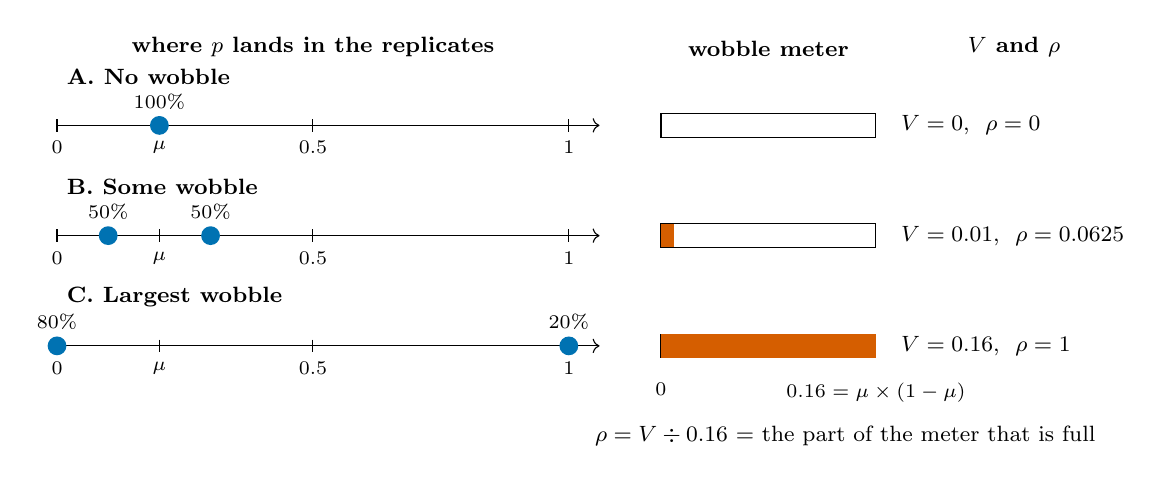
\begin{tikzpicture}[x=6.5cm,y=1cm,font=\small,
  dot/.style={circle,fill=barcsblue,inner sep=2.4pt}]
  \def\mx{1.18}   % x start of meter
  \def\mw{0.42}   % meter width (full = 0.16)
  \node[font=\footnotesize\bfseries,anchor=south] at (0.5,3.75) {where $p$ lands in the replicates};
  \node[font=\footnotesize\bfseries,anchor=south] at (\mx+\mw/2,3.75)
    {wobble meter};
  \node[font=\footnotesize\bfseries,anchor=south] at (\mx+\mw+0.27,3.75) {$V$ and $\rho$};
  \foreach \y/\name in {3/{A. No wobble}, 1.6/{B. Some wobble}, 0.2/{C. Largest wobble}} {
    \draw[->] (0,\y) -- (1.06,\y);
    \foreach \t in {0,0.2,0.5,1} \draw (\t,\y+0.08) -- (\t,\y-0.08);
    \node[font=\scriptsize,below] at (0,\y-0.08) {0};
    \node[font=\scriptsize,below] at (0.2,\y-0.08) {$\mu$};
    \node[font=\scriptsize,below] at (0.5,\y-0.08) {0.5};
    \node[font=\scriptsize,below] at (1,\y-0.08) {1};
    \node[anchor=west,font=\footnotesize\bfseries] at (0,\y+0.62) {\name};
    \draw (\mx,\y-0.15) rectangle (\mx+\mw,\y+0.15);
  }
  % A: all replicates at mu
  \node[dot] at (0.2,3) {}; \node[font=\scriptsize,above] at (0.2,3.08) {100\%};
  \node[anchor=west,font=\footnotesize] at (\mx+\mw+0.03,3) {$V = 0$, \ $\rho = 0$};
  % B: 0.1 or 0.3
  \node[dot] at (0.1,1.6) {}; \node[font=\scriptsize,above] at (0.1,1.68) {50\%};
  \node[dot] at (0.3,1.6) {}; \node[font=\scriptsize,above] at (0.3,1.68) {50\%};
  \fill[barcsorange] (\mx,1.45) rectangle (\mx+\mw*0.0625,1.75);
  \node[anchor=west,font=\footnotesize] at (\mx+\mw+0.03,1.6) {$V = 0.01$, \ $\rho = 0.0625$};
  % C: 0 or 1
  \node[dot] at (0,0.2) {}; \node[font=\scriptsize,above] at (0,0.28) {80\%};
  \node[dot] at (1,0.2) {}; \node[font=\scriptsize,above] at (1,0.28) {20\%};
  \fill[barcsorange] (\mx,0.05) rectangle (\mx+\mw,0.35);
  \node[anchor=west,font=\footnotesize] at (\mx+\mw+0.03,0.2) {$V = 0.16$, \ $\rho = 1$};
  % meter scale
  \node[font=\scriptsize,below] at (\mx,-0.15) {0};
  \node[font=\scriptsize,below] at (\mx+\mw,-0.15) {$0.16 = \mu \times (1-\mu)$};
  \node[font=\footnotesize,align=center] at (\mx+\mw/2+0.15,-0.95)
    {$\rho = V \div 0.16$ = the part of the meter that is full};
\end{tikzpicture}
}
\end{center}
\begin{itemize}\small
\item No wobble: reads unrelated, $\rho = 0$. Largest wobble ($p$ is 0 or 1):
  both reads always the same, $\rho = 1$.
\item The largest possible wobble is $\mu \times (1-\mu)$ (next slide).
\end{itemize}
\end{frame}

\begin{frame}{Why $\rho$ is never more than 1}
\small
\renewcommand{\arraystretch}{1.15}
\begin{tabular}{@{}r@{\;}l l l@{}}
\toprule
& Rule & Case B ($p = 0.1, 0.3$) & Case C ($p = 0, 1$)\\
\midrule
a. & $V = $ avg.\ of $p^2 - \mu^2$ & $0.05 - 0.04 = 0.01$ & $0.2 - 0.04 = 0.16$\\
b. & $p \times p \le p$ when $0 \le p \le 1$ & $0.01 \le 0.1$,\ $0.09 \le 0.3$ & $0 = 0$,\ $1 = 1$\\
c. & so: avg.\ of $p^2 \le \mu$ & $0.05 \le 0.2$ & $0.2 = 0.2$\\
d. & so: $V \le \mu - \mu^2 = \mu \times (1-\mu)$ & $0.01 \le 0.16$ & $0.16 = 0.16$\\
\bottomrule
\end{tabular}

\smallskip
\begin{itemize}\footnotesize
\item a: open $(p-\mu)^2 = p^2 - 2\times\mu\times p + \mu^2$ and average;
  the average of $p$ is $\mu$.
\item b: a number from 0 to 1 does not grow when multiplied by itself
  ($0.3 \times 0.3 = 0.09$).
\item c: every $p^2 \le p$, so the average of $p^2 \le$ the average of $p = \mu$.
\quad d: put c into a.
\end{itemize}
\normalsize
The wobble can never pass $\mu \times (1-\mu)$, so $\rho \le 1$. It reaches
1 only when every $p$ is 0 or 1 (case C).
\end{frame}

\begin{frame}{Turn the formula around}
Multiply both sides by $\mu \times (1-\mu)$:
\[
\rho = \frac{V}{\mu \times (1-\mu)}
\quad\Longrightarrow\quad
\text{covariance of two reads} = V = \rho \times \mu \times (1-\mu)
\]
\begin{worked}[ 4d]
\textbf{Case B:} $0.0625 \times 0.2 \times 0.8 = 0.0625 \times 0.16 = 0.01 = V$.\\[2pt]
\textbf{Our guide:} variance of one read $= 0.000191 \times 0.999809 =
0.000191$; $\rho = 0.000000386$ (two reads almost unrelated);
$V = 0.000000386 \times 0.000191 = 0.0000000000737$; $\sqrt{V} = 8.6$ per
million.
\end{worked}
We use $V = \rho \times \mu \times (1-\mu)$ in Part 4.
\end{frame}

\begin{frame}{Part 4: add up the reads --- two reads first}
The count is a sum: $K = X_1 + X_2 + \dots + X_N$ (each $X$ is 1 or 0).
\medskip

Distance of the sum $=$ sum of the distances. Square it:
\[
(d_1 + d_2)^2 = d_1 \times d_1 + d_2 \times d_2 + 2 \times d_1 \times d_2
\]
Average each part:
\[
\text{variance of } (X_1 + X_2) = \text{variance} + \text{variance} + 2 \times \text{covariance}
\]
\begin{worked}[ 4e: case B]
$0.16 + 0.16 + 2 \times 0.01 = 0.34$.\quad Computer, 100{,}000 pairs: 0.340.
\end{worked}
{\small Independent reads: covariance $= 0$, and we get Part 2, Step B again.}
\end{frame}

\begin{frame}{$N$ reads: squares and pairs}
\vspace{-0.3em}
Square $(d_1 + d_2 + \dots + d_N)$: multiply every part by every part.
\begin{itemize}
\item \textbf{Squares} $d_1 \times d_1, \dots$: $N$ of them, each
  $\mu \times (1-\mu)$ on average.
\item \textbf{Pairs} $d_1 \times d_2, \dots$: each read pairs with the
  $N-1$ others $\Rightarrow$ \alert{$N \times (N-1)$ pairs}, each $V$ on
  average.
\end{itemize}
{\small $N = 3$: pairs 1--2, 1--3, 2--1, 2--3, 3--1, 3--2 $= 6 = 3 \times 2$.
\quad $N = 2$: $2 \times 1 = 2$ pairs (the ``$2\times$'' before).}
\[
\text{variance} = \underbrace{N \times \mu \times (1-\mu)}_{N \text{ squares}}
 + \underbrace{N \times (N-1) \times V}_{N \times (N-1) \text{ pairs}}
\]
\begin{remember}
$N \times (N-1)$ is the \alert{number of pairs of reads} (not $N \times N$:
a read does not pair with itself).
\end{remember}
\end{frame}

\begin{frame}{How $\rho$ gets into the variance formula}
\newcommand{\cV}{\textcolor{barcsorange}{V}}
\newcommand{\cR}{\textcolor{barcsblue}{\rho}}
\footnotesize
\renewcommand{\arraystretch}{1.12}\setlength{\tabcolsep}{4pt}
\begin{tabular}{@{}l l l@{}}
\toprule
\textbf{Step} & \textbf{Formula} & \textbf{Case B, $N = 10$}\\
\midrule
1. Wobble & $\cV = $ average of $(p-\mu)^2$ & $\cV = 0.01$\\
2. Covariance & (both our guide) $- \mu \times \mu = \cV$ & $0.05 - 0.04 = 0.01$\\
3. Correlation & $\cR = \cV \div \bigl(\mu \times (1-\mu)\bigr)$ & $0.01 \div 0.16 = 0.0625$\\
4. Turn around & $\cV = \cR \times \mu \times (1-\mu)$ & $0.0625 \times 0.16 = 0.01$\\
5. Add $N$ reads & $N \times \mu \times (1-\mu) + N \times (N-1) \times \cV$ & $1.6 + 90 \times 0.01 = 2.5$\\
6. Replace $\cV$ & $N \times \mu \times (1-\mu) + N \times (N-1) \times \cR \times \mu \times (1-\mu)$ & $1.6 + 90 \times 0.0625 \times 0.16 = 2.5$\\
7. Take out & $N \times \mu \times (1-\mu) \times \bigl(1 + (N-1) \times \cR\bigr)$ & $1.6 \times 1.5625 = 2.5$\\
\bottomrule
\end{tabular}

\smallskip
{\footnotesize $N \times \mu \times (1-\mu) = 10 \times 0.2 \times 0.8 = 1.6$;\quad
$N \times (N-1) = 10 \times 9 = 90$;\quad $1 + 9 \times 0.0625 = 1.5625$.}

\medskip
\small Step 7 takes out the common part $N \times \mu \times (1-\mu)$. In
step 6, the orange \textcolor{barcsorange}{$V$} is replaced by
\textcolor{barcsblue}{$\rho$}$\,\times \mu \times (1-\mu)$ from step 4.
Every line gives the same number.
\end{frame}

\begin{frame}{Check with ten reads, and our guide}
\begin{worked}[ 4f: ten reads in case B]
Squares $10 \times 0.16 = 1.6$; pairs $90 \times 0.01 = 0.9$; total
$\mathbf{2.5}$.\quad Boxed: $1.6 \times 1.5625 = \mathbf{2.5}$.\\
Computer, 100{,}000 replicates: 2.498.\quad With $N \times N$: 2.6 (wrong).
\end{worked}
\begin{worked}[ 4g: our guide]
Squares $1{,}000{,}000 \times 0.000191 \times 0.999809 = 191.0$; pairs
$1{,}000{,}000 \times 999{,}999 \times 0.0000000000737 = 73.7$.\\
Total $264.7$.\quad Boxed: $191 \times 1.386 = 264.7$.\quad SD
$\sqrt{264.7} = 16.3$ reads.\\
Counting noise alone: $\sqrt{191} = 13.8$. Biological noise adds 39\% to
the variance.
\end{worked}
\end{frame}

\begin{frame}{More reads do not remove biological noise}
\begin{remember}
The extra factor $1 + (N-1) \times \rho$ contains $N$.

When the machine reads more, $N$ grows, and the factor grows too.

So more reading does not remove biological noise. Only \alert{more
replicates} help.
\end{remember}
\end{frame}

%=====================================================================
\section{Step 5: The design matrix}
%=====================================================================

\begin{frame}{What a design matrix is}
\begin{columns}[T]
\begin{column}{0.5\textwidth}
A \alert{design matrix} $X$ is a table of numbers:
\begin{itemize}
\item one \alert{row} for each library
\item one \alert{column} for each $\beta$ value
\end{itemize}
\medskip
\centering
\begin{tabular}{lc|cc}
\toprule
Lib. & Group & Intercept & Drug\\
\midrule
1 & control & 1 & 0\\
2 & control & 1 & 0\\
3 & drug    & 1 & 1\\
4 & drug    & 1 & 1\\
\bottomrule
\end{tabular}
\end{column}
\begin{column}{0.46\textwidth}
\begin{symbols}
\small
\textbf{Intercept}: a column of 1s. It belongs to $\beta_0$, the starting
level.

\textbf{Drug}: 1 for a drug library, 0 for control. It belongs to
$\beta_1$.

$\beta_0$: the control log-odds.

$\beta_1$: the change from control to drug. This is the \alert{effect}.
\end{symbols}
\end{column}
\end{columns}
\end{frame}

\begin{frame}{From the design matrix to a prediction}
Take the row of a library. Multiply each number by its $\beta$. Add:
\[
\eta = (\text{column 1}) \times \beta_0 + (\text{column 2}) \times \beta_1
\]
\begin{worked}[ 5: predictions]
BARCS finds $\beta_0 = -8.565$ and $\beta_1 = -0.542$ (Step 6 in
Chapter~2).

\begin{tabular}{@{}lll@{}}
Libraries 1, 2 (row 1, 0): & $1 \times (-8.565) + 0 \times (-0.542)$ & $= -8.565$\\
Libraries 3, 4 (row 1, 1): & $1 \times (-8.565) + 1 \times (-0.542)$ & $= -9.107$\\
\end{tabular}

Control gets $\beta_0$. Drug gets $\beta_0 + \beta_1$. So $\beta_1$ is the
difference.
\end{worked}
\end{frame}

\begin{frame}{From log-odds back to counts}
\[
\mu = \frac{e^{\eta}}{1 + e^{\eta}}, \qquad \text{expected count} = N \times \mu
\]
\begin{worked}[ 6: expected counts]
\small
Control: $e^{-8.565} = 0.000190676$, so $\mu = 0.000190640$ (190.6 per
million). Drug: $\mu = 0.000110827$ (110.8 per million).

\begin{tabular}{@{}lrrrr@{}}
\toprule
Library & $N$ & $\mu$ (per million) & Expected $N \times \mu$ & Real $K$\\
\midrule
1 & 1{,}000{,}000 & 190.6 & 190.6 & 180\\
2 & 1{,}200{,}000 & 190.6 & 228.8 & 240\\
3 & 1{,}000{,}000 & 110.8 & 110.8 & 120\\
4 &   800{,}000 & 110.8 &  88.7 &  80\\
\bottomrule
\end{tabular}

The differences ($-10.6$, $+11.2$, $+9.2$, $-8.7$) are the noise.
\end{worked}
\end{frame}

\begin{frame}{The reference group}
\begin{itemize}
\item Control has 0 in the drug column. So control is the
  \alert{reference group}.
\item $\beta_1$ always compares a group with the reference group.
\item If drug becomes the reference group, $\beta_1$ changes sign:
  $+0.542$. The meaning stays the same.
\end{itemize}
\end{frame}

\begin{frame}{Paired replicates: add a column}
\begin{columns}[T]
\begin{column}{0.5\textwidth}
\small
If replicate 1 of control and drug come from the same batch, add a batch
column:

\medskip
\begin{tabular}{lc|ccc}
\toprule
Lib. & Rep. & Int. & Rep.\,2 & Drug\\
\midrule
1 & 1 & 1 & 0 & 0\\
2 & 2 & 1 & 1 & 0\\
3 & 1 & 1 & 0 & 1\\
4 & 2 & 1 & 1 & 1\\
\bottomrule
\end{tabular}

\medskip
Each new column costs one degree of freedom.
\end{column}
\begin{column}{0.46\textwidth}
\begin{worked}[ 7: the paired model]
\small
Drug effect: $\beta = -0.544$, SE 0.143.

Degrees of freedom: $4 - 3 = 1$ (was 2).

p-value: 0.164 (was 0.033).

The batch difference is only 0.005. The column costs information and gives
nothing back.
\end{worked}
\end{column}
\end{columns}
\end{frame}

\begin{frame}{Numbers instead of groups: a time course}
\begin{columns}[T]
\begin{column}{0.44\textwidth}
\centering
\begin{tabular}{lc|cc}
\toprule
Lib. & Day & Int. & Day $\div$ 14\\
\midrule
1, 2 & 0  & 1 & 0\\
3, 4 & 7  & 1 & 0.5\\
5, 6 & 14 & 1 & 1\\
\bottomrule
\end{tabular}

\medskip
\raggedright\small $\beta_1$ is the change in log-odds over 14 days.
\end{column}
\begin{column}{0.52\textwidth}
\begin{worked}[ 8: a time course]
\small
Suppose $\beta_1 = -0.70$.

Day 14: $1 \times (-0.70) = -0.70$; $e^{-0.70} = 0.50$. Half.

Day 7: $0.5 \times (-0.70) = -0.35$; $e^{-0.35} = 0.70$. 70\%.

Degrees of freedom: $6 - 2 = 4$.
\end{worked}
\end{column}
\end{columns}
\end{frame}

\begin{frame}{Two factors and an interaction}
\begin{center}
\begin{tabular}{l|cccc}
\toprule
Group & Intercept & Knockout & Drug & Knockout $\times$ Drug\\
\midrule
normal, no drug   & 1 & 0 & 0 & 0\\
knockout, no drug & 1 & 1 & 0 & 0\\
normal, drug      & 1 & 0 & 1 & 0\\
knockout, drug    & 1 & 1 & 1 & 1\\
\bottomrule
\end{tabular}
\end{center}
\begin{itemize}
\item The last column is knockout $\times$ drug. It is 1 only when both are
  1.
\item Its $\beta$ is the \alert{interaction}: the extra change that happens
  only when both changes happen together.
\end{itemize}
\end{frame}

\begin{frame}{Worked example: reading an interaction}
\begin{worked}[ 9]
The four $\beta$ values are $-8.5$, $-0.2$, $+0.1$ and $-0.7$.

\begin{tabular}{@{}ll@{}}
normal, no drug:   & $-8.5$\\
knockout, no drug: & $-8.5 + (-0.2) = -8.7$\\
normal, drug:      & $-8.5 + 0.1 = -8.4$\\
knockout, drug:    & $-8.5 + (-0.2) + 0.1 + (-0.7) = -9.3$\\
\end{tabular}

If the effects only added up: $-8.5 - 0.2 + 0.1 = -8.6$. The real value
is $-9.3$. The extra $-0.7$ is the interaction.
\end{worked}
\end{frame}

\begin{frame}{Comparing two treatments: a contrast}
\begin{itemize}
\item Three groups: control, drug A, drug B.
\item $\beta_A$ compares drug A with control. $\beta_B$ compares drug B with
  control.
\item To compare drug A with drug B, subtract: $\beta_A - \beta_B$. This is
  a \alert{contrast}.
\item In BARCS: \texttt{bb\_contrast()}.
\end{itemize}
\medskip
Example: $\beta_A = -0.9$, $\beta_B = -0.4$, so
$\beta_A - \beta_B = -0.5$. Drug A lowers the guide more.
\end{frame}

\begin{frame}{Rules for a good design matrix}
\begin{enumerate}
\item One row for each library, in the order of the count table.
\item One column for each $\beta$ that you want.
\item More rows than columns. The difference is the degrees of freedom.
  Two or more is better than one.
\item No two columns with the same information.
\end{enumerate}
\medskip
\begin{remember}
Suppose all drug libraries come from batch 2 and all control libraries from
batch 1. Then the batch column equals the drug column. BARCS cannot
separate the drug effect from the batch effect.
\end{remember}
\end{frame}

\begin{frame}[fragile]{The design matrix in R}
\small A \alert{formula} describes $X$. \texttt{model.matrix()} builds it:
\footnotesize
\begin{verbatim}
> data <- data.frame(group = c("control", "control", "drug", "drug"))
> model.matrix(~ group, data)
  (Intercept) groupdrug
1           1         0
2           1         0
3           1         1
4           1         1
\end{verbatim}
\small Then give BARCS the counts, totals, formula and column name:
\footnotesize
\begin{verbatim}
fit <- bb_screen(counts, data, formula = ~ group,
                 term = "groupdrug", totals = totals)
\end{verbatim}
\small Paired: \texttt{\textasciitilde\ replicate + group}.\quad
Interaction: \texttt{\textasciitilde\ knockout * drug}.
\end{frame}

%=====================================================================
\section{Chapter 1 summary}
%=====================================================================

\begin{frame}{What Chapter 1 showed}
\begin{enumerate}
\item BARCS turns read counts into proportions (Step 1).
\item It compares groups with a fold change and its logarithm (Step 2).
\item It works on the log-odds scale (Step 3).
\item It separates counting noise from biological noise (Step 4).
\item It describes the experiment with a design matrix (Step 5).
\end{enumerate}
\medskip
\alert{Chapter 2} shows how BARCS calculates the effect and decides if it
is real.
\end{frame}

\begin{frame}{The symbols of Chapter 1}
\centering\footnotesize\renewcommand{\arraystretch}{0.95}
\begin{tabular}{@{}lll@{}}
\toprule
Symbol & Meaning & Value in our example\\
\midrule
$K$ & read count of the guide in one library & 180, 240, 120, 80\\
$N$ & total read count of one library & 1.0, 1.2, 1.0, 0.8 million\\
$p$ & proportion, $K/N$ & 191 and 111 per million\\
fold change & $p_{\text{drug}} \div p_{\text{control}}$ & 0.58\\
$\log_2$, $\ln$ & doublings; powers of $e$ & $-0.78$; $-0.54$\\
log-odds & $\ln\bigl(p/(1-p)\bigr)$ & $-8.56$ (control)\\
$\mu$ & expected proportion & 0.000191 (control)\\
$\rho$ & biological noise & 0.000000386\\
$X$ & design matrix: a row per library, a column per $\beta$ & 4 rows, 2 columns\\
$\beta_0$, $\beta_1$ & control log-odds; effect of the drug & $-8.565$; $-0.542$\\
$\eta$ & predicted log-odds (row of $X$ times $\beta$) & $-8.565$, $-9.107$\\
\bottomrule
\end{tabular}
\end{frame}

\end{document}
